\documentclass[11pt]{article}
\usepackage[utf8]{inputenc}
\usepackage{amsmath}
\usepackage{amsfonts}
\usepackage{amssymb}
\usepackage{geometry}
\usepackage{enumitem}
\usepackage{graphicx}
\usepackage{tikz}
\usepackage{pgfplots}
\usepackage{amsthm}
\usepackage{mathtools}
\usepackage{tikz-3dplot}

\geometry{margin=1in}

\theoremstyle{definition}
\newtheorem{definition}{Definition}[section]
\newtheorem{theorem}{Theorem}[section]
\newtheorem{lemma}{Lemma}[section]
\newtheorem{corollary}{Corollary}[section]
\newtheorem{example}{Example}[section]
\newtheorem{proposition}{Proposition}[section]

\title{Differential Geometry Summary}
\author{Mathematical Notes}
\date{\today}

\begin{document}

\maketitle

\tableofcontents
\newpage

\section{Manifolds}

\subsection{Definition and Basic Properties}
\begin{definition}
A \textbf{topological manifold} of dimension $n$ is a topological space $M$ such that:
\begin{enumerate}
    \item $M$ is Hausdorff
    \item $M$ is second countable
    \item Every point $p \in M$ has a neighborhood homeomorphic to an open subset of $\mathbb{R}^n$
\end{enumerate}
\end{definition}

\begin{definition}
A \textbf{smooth manifold} is a topological manifold equipped with a smooth atlas, i.e., a collection of charts $(U_\alpha, \phi_\alpha)$ such that the transition maps $\phi_\beta \circ \phi_\alpha^{-1}$ are smooth.
\end{definition}

\subsection{Examples of Manifolds}
\begin{example}
\begin{itemize}
    \item $\mathbb{R}^n$ is an $n$-dimensional manifold
    \item $S^n = \{x \in \mathbb{R}^{n+1} : |x| = 1\}$ is an $n$-dimensional sphere
    \item The torus $T^2 = S^1 \times S^1$ is a 2-dimensional manifold
    \item The projective plane $\mathbb{RP}^2$ is a 2-dimensional manifold
\end{itemize}
\end{example}

% Illustration of a manifold
\begin{figure}[h]
\centering
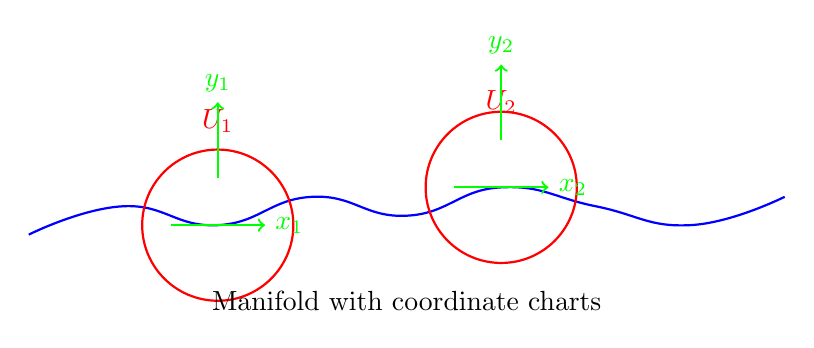
\begin{tikzpicture}[scale=1.2]
    % Draw a wavy surface representing a manifold
    \draw[thick, blue] plot[smooth, tension=0.8] coordinates {
        (0,0) (1,0.3) (2,0.1) (3,0.4) (4,0.2) (5,0.5) (6,0.3) (7,0.1) (8,0.4)
    };
    
    % Draw coordinate patches
    \draw[red, thick] (2,0.1) circle (0.8);
    \draw[red, thick] (5,0.5) circle (0.8);
    
    % Label the patches
    \node[red] at (2,1.2) {$U_1$};
    \node[red] at (5,1.4) {$U_2$};
    
    % Draw coordinate axes in patches
    \draw[green, thick, ->] (1.5,0.1) -- (2.5,0.1) node[right] {$x_1$};
    \draw[green, thick, ->] (2,0.6) -- (2,1.4) node[above] {$y_1$};
    
    \draw[green, thick, ->] (4.5,0.5) -- (5.5,0.5) node[right] {$x_2$};
    \draw[green, thick, ->] (5,1.0) -- (5,1.8) node[above] {$y_2$};
    
    \node[below] at (4,-0.5) {Manifold with coordinate charts};
\end{tikzpicture}
\caption{A manifold with overlapping coordinate charts}
\end{figure}

\section{Tangent Spaces and Vectors}

\subsection{Tangent Vectors}
\begin{definition}
A \textbf{tangent vector} at point $p \in M$ is an equivalence class of smooth curves $\gamma: (-\epsilon, \epsilon) \to M$ with $\gamma(0) = p$, where two curves are equivalent if they have the same derivative in any coordinate chart.
\end{definition}

\begin{definition}
The \textbf{tangent space} $T_pM$ at point $p$ is the vector space of all tangent vectors at $p$.
\end{definition}

\subsection{Tangent Bundle}
\begin{definition}
The \textbf{tangent bundle} $TM$ is the disjoint union of all tangent spaces:
$$TM = \bigcup_{p \in M} T_pM$$
\end{definition}

% Illustration of tangent space
\begin{figure}[h]
\centering
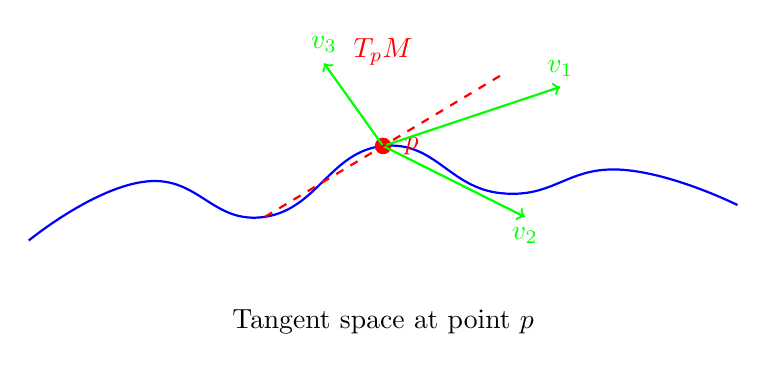
\begin{tikzpicture}[scale=1.5]
    % Draw a curve (manifold)
    \draw[thick, blue] plot[smooth, tension=0.8] coordinates {
        (0,0) (1,0.5) (2,0.2) (3,0.8) (4,0.4) (5,0.6) (6,0.3)
    };
    
    % Mark a point
    \fill[red] (3,0.8) circle (2pt);
    \node[red, right] at (3.1,0.8) {$p$};
    
    % Draw tangent vectors
    \draw[green, thick, ->] (3,0.8) -- (4.5,1.3) node[above] {$v_1$};
    \draw[green, thick, ->] (3,0.8) -- (4.2,0.2) node[below] {$v_2$};
    \draw[green, thick, ->] (3,0.8) -- (2.5,1.5) node[above] {$v_3$};
    
    % Draw tangent space
    \draw[red, dashed, thick] (2,0.2) -- (4,1.4);
    \node[red, above] at (3,1.4) {$T_pM$};
    
    \node[below] at (3,-0.5) {Tangent space at point $p$};
\end{tikzpicture}
\caption{Tangent vectors and tangent space}
\end{figure}

\section{Vector Fields}

\subsection{Definition}
\begin{definition}
A \textbf{vector field} on manifold $M$ is a smooth assignment of a tangent vector to each point of $M$.
\end{definition}

\subsection{Lie Bracket}
\begin{definition}
The \textbf{Lie bracket} of vector fields $X$ and $Y$ is the vector field $[X,Y]$ defined by:
$$[X,Y]f = X(Yf) - Y(Xf)$$
for any smooth function $f$.
\end{definition}

% Illustration of vector field
\begin{figure}[h]
\centering
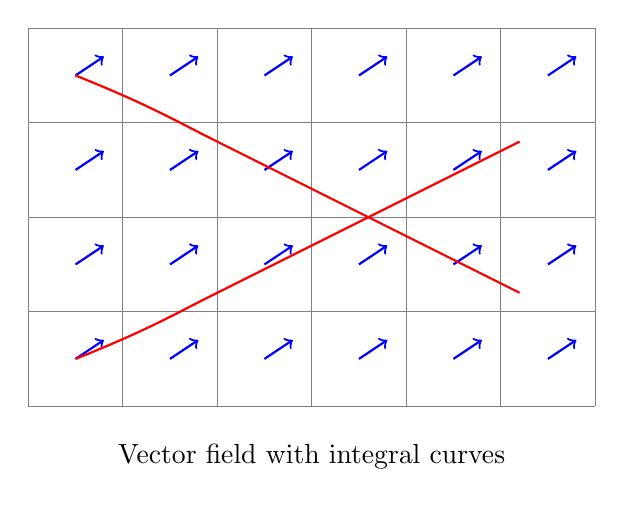
\begin{tikzpicture}[scale=1.2]
    % Draw a grid
    \draw[gray, thin] (0,0) grid (6,4);
    
    % Draw vector field
    \foreach \x in {0.5,1.5,2.5,3.5,4.5,5.5}
        \foreach \y in {0.5,1.5,2.5,3.5} {
            \draw[blue, thick, ->] (\x,\y) -- (\x+0.3,\y+0.2);
        }
    
    % Draw some integral curves
    \draw[red, thick] plot[smooth, tension=0.8] coordinates {
        (0.5,0.5) (1.2,0.8) (2.0,1.2) (2.8,1.6) (3.6,2.0) (4.4,2.4) (5.2,2.8)
    };
    
    \draw[red, thick] plot[smooth, tension=0.8] coordinates {
        (0.5,3.5) (1.2,3.2) (2.0,2.8) (2.8,2.4) (3.6,2.0) (4.4,1.6) (5.2,1.2)
    };
    
    \node[below] at (3,-0.3) {Vector field with integral curves};
\end{tikzpicture}
\caption{Vector field and its integral curves}
\end{figure}

\section{Differential Forms}

\subsection{Definition}
\begin{definition}
A \textbf{differential $k$-form} on manifold $M$ is a smooth assignment of an alternating $k$-linear form on each tangent space.
\end{definition}

\subsection{Exterior Derivative}
\begin{definition}
The \textbf{exterior derivative} $d$ is a linear operator on differential forms satisfying:
\begin{enumerate}
    \item $d^2 = 0$
    \item $d(\omega \wedge \eta) = d\omega \wedge \eta + (-1)^k \omega \wedge d\eta$
    \item For functions $f$, $df$ is the usual differential
\end{enumerate}
\end{definition}

\subsection{Stokes' Theorem}
\begin{theorem}
Let $M$ be an oriented $n$-dimensional manifold with boundary, and let $\omega$ be an $(n-1)$-form. Then:
$$\int_M d\omega = \int_{\partial M} \omega$$
\end{theorem}

\section{Riemannian Geometry}

\subsection{Riemannian Metric}
\begin{definition}
A \textbf{Riemannian metric} on manifold $M$ is a smooth assignment of an inner product on each tangent space.
\end{definition}

\begin{definition}
A \textbf{Riemannian manifold} is a smooth manifold equipped with a Riemannian metric.
\end{definition}

\subsection{Length and Distance}
\begin{definition}
The \textbf{length} of a curve $\gamma: [a,b] \to M$ is:
$$L(\gamma) = \int_a^b \sqrt{g(\gamma'(t), \gamma'(t))} \, dt$$
\end{definition}

\begin{definition}
The \textbf{distance} between two points is the infimum of lengths of curves connecting them.
\end{definition}

% Illustration of geodesic
\begin{figure}[h]
\centering
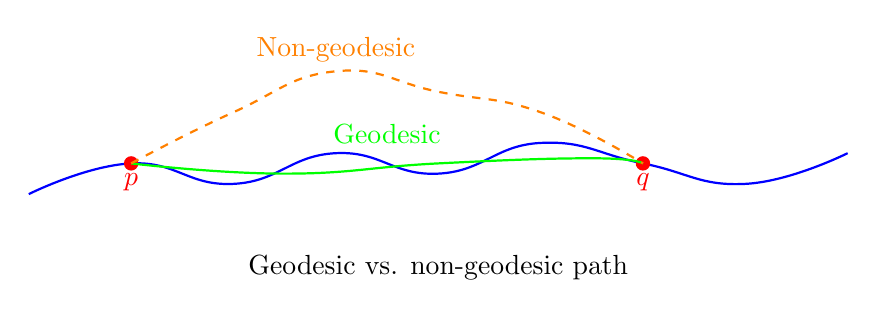
\begin{tikzpicture}[scale=1.3]
    % Draw a curved surface
    \draw[thick, blue] plot[smooth, tension=0.8] coordinates {
        (0,0) (1,0.3) (2,0.1) (3,0.4) (4,0.2) (5,0.5) (6,0.3) (7,0.1) (8,0.4)
    };
    
    % Draw two points
    \fill[red] (1,0.3) circle (2pt);
    \fill[red] (6,0.3) circle (2pt);
    \node[red, below] at (1,0.3) {$p$};
    \node[red, below] at (6,0.3) {$q$};
    
    % Draw geodesic (shortest path)
    \draw[green, thick] plot[smooth, tension=0.8] coordinates {
        (1,0.3) (2.5,0.2) (4,0.3) (5.5,0.35) (6,0.3)
    };
    
    % Draw a non-geodesic path
    \draw[orange, thick, dashed] plot[smooth, tension=0.8] coordinates {
        (1,0.3) (2,0.8) (3,1.2) (4,1.0) (5,0.8) (6,0.3)
    };
    
    \node[green, above] at (3.5,0.4) {Geodesic};
    \node[orange, above] at (3,1.2) {Non-geodesic};
    
    \node[below] at (4,-0.5) {Geodesic vs. non-geodesic path};
\end{tikzpicture}
\caption{Geodesic as shortest path on a curved surface}
\end{figure}

\section{Curvature}

\subsection{Levi-Civita Connection}
\begin{definition}
The \textbf{Levi-Civita connection} is the unique torsion-free, metric-compatible connection on a Riemannian manifold.
\end{definition}

\subsection{Riemann Curvature Tensor}
\begin{definition}
The \textbf{Riemann curvature tensor} is defined by:
$$R(X,Y)Z = \nabla_X \nabla_Y Z - \nabla_Y \nabla_X Z - \nabla_{[X,Y]} Z$$
\end{definition}

\subsection{Scalar and Ricci Curvature}
\begin{definition}
The \textbf{Ricci curvature tensor} is:
$$\text{Ric}(X,Y) = \text{tr}(Z \mapsto R(Z,X)Y)$$
\end{definition}

\begin{definition}
The \textbf{scalar curvature} is the trace of the Ricci tensor.
\end{definition}

% Illustration of curvature
\begin{figure}[h]
\centering
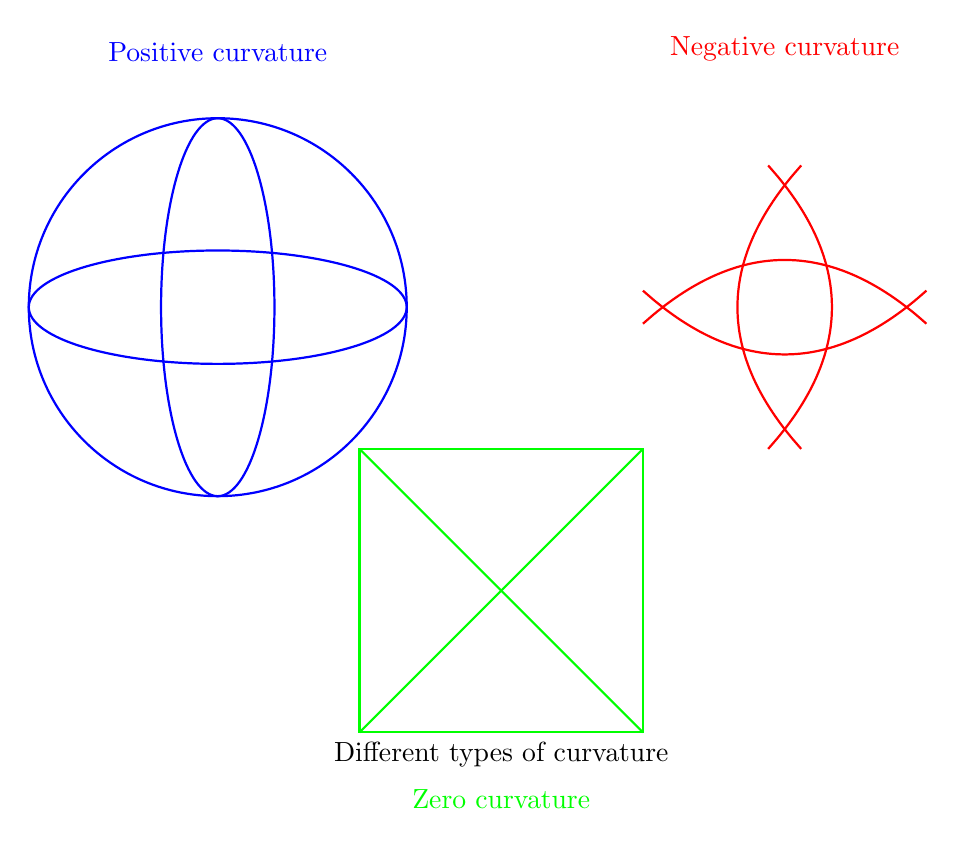
\begin{tikzpicture}[scale=1.2]
    % Draw a sphere (positive curvature)
    \draw[thick, blue] (0,0) circle (2);
    \draw[thick, blue] (0,0) ellipse (2 and 0.6);
    \draw[thick, blue] (0,0) ellipse (0.6 and 2);
    
    \node[blue, above] at (0,2.5) {Positive curvature};
    
    % Draw a saddle (negative curvature)
    \begin{scope}[xshift=6cm]
        \draw[thick, red] plot[smooth, domain=-1.5:1.5] (\x, {0.3*\x*\x - 0.5});
        \draw[thick, red] plot[smooth, domain=-1.5:1.5] (\x, {-0.3*\x*\x + 0.5});
        \draw[thick, red] plot[smooth, domain=-1.5:1.5] ({0.3*\x*\x - 0.5}, \x);
        \draw[thick, red] plot[smooth, domain=-1.5:1.5] ({-0.3*\x*\x + 0.5}, \x);
        
        \node[red, above] at (0,2.5) {Negative curvature};
    \end{scope}
    
    % Draw a plane (zero curvature)
    \begin{scope}[xshift=3cm, yshift=-3cm]
        \draw[thick, green] (-1.5,-1.5) rectangle (1.5,1.5);
        \draw[thick, green] (-1.5,-1.5) -- (1.5,1.5);
        \draw[thick, green] (-1.5,1.5) -- (1.5,-1.5);
        
        \node[green, below] at (0,-2) {Zero curvature};
    \end{scope}
    
    \node[below] at (3,-4.5) {Different types of curvature};
\end{tikzpicture}
\caption{Positive, negative, and zero curvature surfaces}
\end{figure}

\section{Geodesics}

\subsection{Definition}
\begin{definition}
A \textbf{geodesic} is a curve whose tangent vector is parallel transported along itself.
\end{definition}

\subsection{Geodesic Equation}
\begin{theorem}
A curve $\gamma(t)$ is a geodesic if and only if it satisfies the geodesic equation:
$$\frac{d^2 \gamma^k}{dt^2} + \Gamma_{ij}^k \frac{d\gamma^i}{dt} \frac{d\gamma^j}{dt} = 0$$
where $\Gamma_{ij}^k$ are the Christoffel symbols.
\end{theorem}

\section{Submanifolds}

\subsection{Definition}
\begin{definition}
A \textbf{submanifold} of manifold $M$ is a subset $N \subseteq M$ that is itself a manifold with the induced topology and smooth structure.
\end{definition}

\subsection{Embedding and Immersion}
\begin{definition}
A smooth map $f: N \to M$ is an \textbf{embedding} if it is a diffeomorphism onto its image.
\end{definition}

\begin{definition}
A smooth map $f: N \to M$ is an \textbf{immersion} if its derivative is injective at every point.
\end{definition}

% Illustration of submanifold
\begin{figure}[h]
\centering
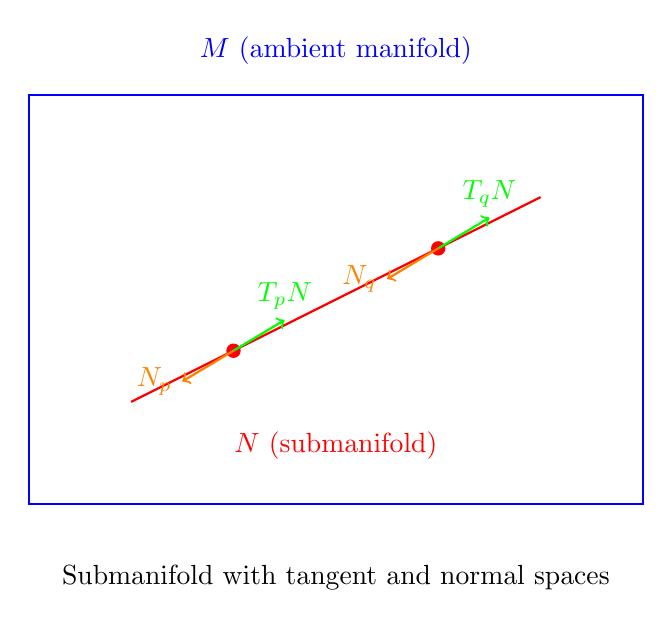
\begin{tikzpicture}[scale=1.3]
    % Draw the ambient manifold (3D space)
    \draw[thick, blue] (0,0) -- (6,0) -- (6,4) -- (0,4) -- cycle;
    
    % Draw a submanifold (curve)
    \draw[thick, red] plot[smooth, tension=0.8] coordinates {
        (1,1) (2,1.5) (3,2) (4,2.5) (5,3)
    };
    
    % Mark points on the submanifold
    \fill[red] (2,1.5) circle (2pt);
    \fill[red] (4,2.5) circle (2pt);
    
    % Draw tangent vectors to the submanifold
    \draw[green, thick, ->] (2,1.5) -- (2.5,1.8) node[above] {$T_pN$};
    \draw[green, thick, ->] (4,2.5) -- (4.5,2.8) node[above] {$T_qN$};
    
    % Draw normal vectors
    \draw[orange, thick, ->] (2,1.5) -- (1.5,1.2) node[left] {$N_p$};
    \draw[orange, thick, ->] (4,2.5) -- (3.5,2.2) node[left] {$N_q$};
    
    \node[blue, above] at (3,4.2) {$M$ (ambient manifold)};
    \node[red, below] at (3,0.8) {$N$ (submanifold)};
    
    \node[below] at (3,-0.5) {Submanifold with tangent and normal spaces};
\end{tikzpicture}
\caption{Submanifold with tangent and normal vectors}
\end{figure}

\section{Lie Groups}

\subsection{Definition}
\begin{definition}
A \textbf{Lie group} is a smooth manifold that is also a group, where the group operations are smooth.
\end{definition}

\subsection{Lie Algebra}
\begin{definition}
The \textbf{Lie algebra} of a Lie group $G$ is the tangent space at the identity $T_eG$ equipped with the Lie bracket.
\end{definition}

\subsection{Examples}
\begin{example}
\begin{itemize}
    \item $GL(n,\mathbb{R})$ - general linear group
    \item $SO(n)$ - special orthogonal group
    \item $SU(n)$ - special unitary group
    \item $S^1$ - circle group
\end{itemize}
\end{example}

\section{Fiber Bundles}

\subsection{Definition}
\begin{definition}
A \textbf{fiber bundle} is a quadruple $(E, B, F, \pi)$ where:
\begin{itemize}
    \item $E$ is the total space
    \item $B$ is the base space
    \item $F$ is the fiber
    \item $\pi: E \to B$ is the projection map
\end{itemize}
\end{definition}

\subsection{Vector Bundles}
\begin{definition}
A \textbf{vector bundle} is a fiber bundle where each fiber is a vector space and the transition functions are linear.
\end{definition}

% Illustration of fiber bundle
\begin{figure}[h]
\centering
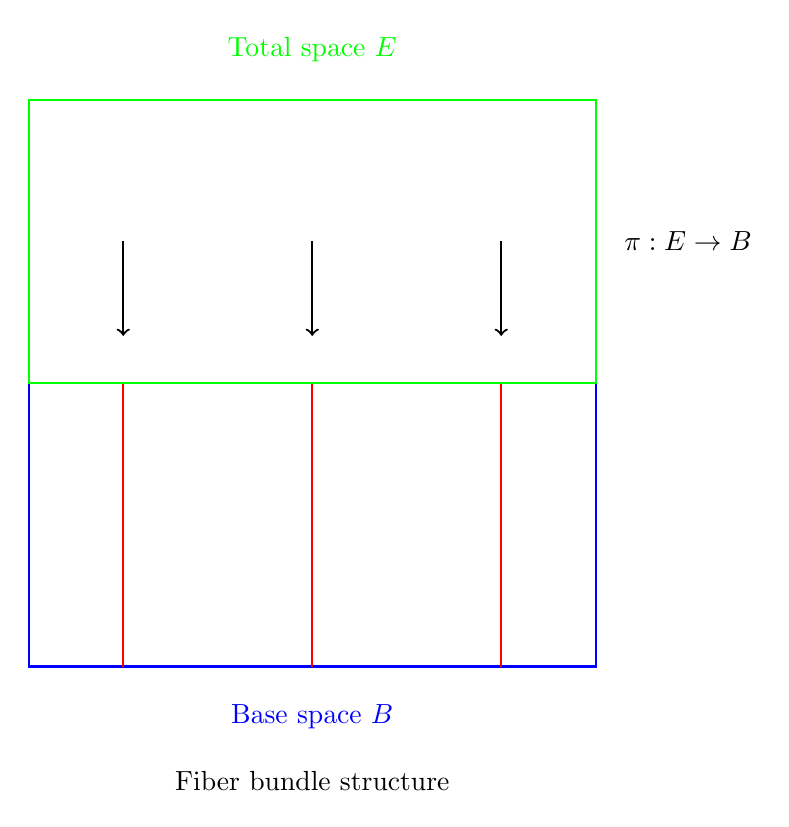
\begin{tikzpicture}[scale=1.2]
    % Draw the base space
    \draw[thick, blue] (0,0) -- (6,0) -- (6,3) -- (0,3) -- cycle;
    \node[blue, below] at (3,-0.3) {Base space $B$};
    
    % Draw fibers at different points
    \draw[thick, red] (1,0) -- (1,3);
    \draw[thick, red] (3,0) -- (3,3);
    \draw[thick, red] (5,0) -- (5,3);
    
    % Draw the total space
    \draw[thick, green] (0,3) -- (6,3) -- (6,6) -- (0,6) -- cycle;
    \node[green, above] at (3,6.3) {Total space $E$};
    
    % Draw projection arrows
    \draw[thick, ->] (1,4.5) -- (1,3.5);
    \draw[thick, ->] (3,4.5) -- (3,3.5);
    \draw[thick, ->] (5,4.5) -- (5,3.5);
    
    \node[right] at (6.2,4.5) {$\pi: E \to B$};
    
    \node[below] at (3,-1) {Fiber bundle structure};
\end{tikzpicture}
\caption{Fiber bundle with base space, total space, and fibers}
\end{figure}

\section{Applications}

\subsection{Physics}
Differential geometry is fundamental to:
\begin{itemize}
    \item General relativity (spacetime as a Lorentzian manifold)
    \item Gauge theory (fiber bundles)
    \item Classical mechanics (symplectic geometry)
    \item Quantum mechanics (complex manifolds)
\end{itemize}

\subsection{Computer Graphics}
Applications include:
\begin{itemize}
    \item Surface modeling
    \item Mesh processing
    \item Shape analysis
    \item Animation
\end{itemize}

\subsection{Robotics}
Used in:
\begin{itemize}
    \item Configuration spaces
    \item Motion planning
    \item Control theory
    \item Sensor fusion
\end{itemize}

\section{Important Theorems}

\subsection{Gauss-Bonnet Theorem}
\begin{theorem}
For a compact 2-dimensional Riemannian manifold $M$:
$$\int_M K \, dA = 2\pi \chi(M)$$
where $K$ is the Gaussian curvature and $\chi(M)$ is the Euler characteristic.
\end{theorem}

\subsection{Myers' Theorem}
\begin{theorem}
If a complete Riemannian manifold has Ricci curvature bounded below by a positive constant, then it is compact.
\end{theorem}

\subsection{Hopf-Rinow Theorem}
\begin{theorem}
A Riemannian manifold is geodesically complete if and only if it is complete as a metric space.
\end{theorem}

\subsection{Nash Embedding Theorem}
\begin{theorem}
Every Riemannian manifold can be isometrically embedded in some Euclidean space.
\end{theorem}

\section{Advanced Topics}

\subsection{Symplectic Geometry}
\begin{definition}
A \textbf{symplectic manifold} is a smooth manifold equipped with a closed, non-degenerate 2-form.
\end{definition}

\subsection{Complex Geometry}
\begin{definition}
A \textbf{complex manifold} is a manifold with an atlas of charts to $\mathbb{C}^n$ with holomorphic transition functions.
\end{definition}

\subsection{Kähler Manifolds}
\begin{definition}
A \textbf{Kähler manifold} is a complex manifold with a Riemannian metric that is compatible with the complex structure.
\end{definition}

\subsection{Spin Geometry}
\begin{definition}
A \textbf{spin manifold} is a Riemannian manifold that admits a spin structure.
\end{definition}

\end{document}
